% General Tikz Settings
\tikzset{
    base node/.style={circle, draw, minimum size=0.85cm,
    font=\sffamily\bfseries\normalsize, thick},
    derived node/.style={circle, draw, minimum size=0.72cm, inner
    sep=0.75pt, font=\sffamily\small\bfseries, thick, fill=white},
    edge label/.style={font=\sffamily\small, fill=white, inner sep=1.25pt},
}

% Colors used consistently for voltage 0 / 1 / 2 throughout this section
\colorlet{volt0}{blue}
\colorlet{volt1}{red}
\colorlet{volt2}{green!55!black}

% Draw the 3 base nodes on a small equilateral triangle
\newcommand{\drawbase}{
    \node[base node] (u) at (0,0) {\( u \)};
    \node[base node] (v) at (3.4,0) {\( v \)};
    \node[base node] (w) at (1.7,2.94) {\( w \)};
}

% Step 1: invisible coordinates for the 3x3 grid, spaced out to
% reduce edge crowding.
% Edges are drawn against these bare coordinates; the visible node
% circles are drawn
% afterwards (see \drawfibernodes) so that edges never paint over a
% node's fill or label.
\newcommand{\drawfibers}{
    \foreach \name/\x in {u/0, v/3.8, w/7.6} {
        \coordinate (\name0) at (\x, 5.1);
        \coordinate (\name1) at (\x, 2.55);
        \coordinate (\name2) at (\x, 0);
    }
}

% Step 2: the visible fiber labels and node circles, drawn last so
% they sit on top of
% every edge.
\newcommand{\drawfibernodes}{
    \foreach \name/\x in {u/0, v/3.8, w/7.6} {
        \node[font=\sffamily\bfseries\small, text=gray] at (\x, 6.2)
        {Fiber \name};
        \node[derived node, draw=volt0, text=volt0] at (\name0) {\(\name,0\)};
        \node[derived node, draw=volt1, text=volt1] at (\name1) {\(\name,1\)};
        \node[derived node, draw=volt2, text=volt2] at (\name2) {\(\name,2\)};
    }
}

% Draw the undirected intra-fiber loops (lifts of base loops form a
% C_3 in each fiber)
\newcommand{\drawderivedloops}{
    \foreach \name in {u, v, w} {
        \draw[-, thick, black, opacity=0.85] (\name0) to (\name1);
        \draw[-, thick, black, opacity=0.85] (\name1) to (\name2);
        \draw[-, thick, black, opacity=0.85, bend right=40]
        (\name0) to (\name2);
    }
}

\newcommand{\drawlift}[3]{
    % #1 = source fiber, #2 = target fiber, #3 = voltage
    \ifnum#3=0
    \draw[->, >=stealth, thick, volt0, opacity=0.7,
    shorten >=2.2pt, shorten <=2.2pt]
    (#10) to (#20);
    \draw[->, >=stealth, thick, volt0, opacity=0.7,
    shorten >=2.2pt, shorten <=2.2pt]
    (#11) to (#21);
    \draw[->, >=stealth, thick, volt0, opacity=0.7,
    shorten >=2.2pt, shorten <=2.2pt]
    (#12) to (#22);
    \fi
    \ifnum#3=1
    \draw[->, >=stealth, thick, volt1, opacity=0.6,
    shorten >=2.2pt, shorten <=2.2pt]
    (#10) to (#21);
    \draw[->, >=stealth, thick, volt1, opacity=0.6,
    shorten >=2.2pt, shorten <=2.2pt]
    (#11) to (#22);
    \draw[->, >=stealth, thick, volt1, opacity=0.6,
    shorten >=2.2pt, shorten <=2.2pt]
    (#12) to (#20);
    \fi
    \ifnum#3=2
    \draw[->, >=stealth, thick, volt2, opacity=0.6,
    shorten >=2.2pt, shorten <=2.2pt]
    (#10) to (#22);
    \draw[->, >=stealth, thick, volt2, opacity=0.6,
    shorten >=2.2pt, shorten <=2.2pt]
    (#11) to (#20);
    \draw[->, >=stealth, thick, volt2, opacity=0.6,
    shorten >=2.2pt, shorten <=2.2pt]
    (#12) to (#21);
    \fi
}

\newcommand{\drawliftgrey}[3]{
    % #1 = source fiber, #2 = target fiber, #3 = voltage
    \ifnum#3=0
    \draw[->, >=stealth, thick, darkgrey, opacity=0.7,
    shorten >=2.2pt, shorten <=2.2pt]
    (#10) to (#20);
    \draw[->, >=stealth, thick, darkgrey, opacity=0.7,
    shorten >=2.2pt, shorten <=2.2pt]
    (#11) to (#21);
    \draw[->, >=stealth, thick, darkgrey, opacity=0.7,
    shorten >=2.2pt, shorten <=2.2pt]
    (#12) to (#22);
    \fi
    \ifnum#3=1
    \draw[->, >=stealth, thick, darkgrey, opacity=0.6,
    shorten >=2.2pt, shorten <=2.2pt]
    (#10) to (#21);
    \draw[->, >=stealth, thick, darkgrey, opacity=0.6,
    shorten >=2.2pt, shorten <=2.2pt]
    (#11) to (#22);
    \draw[->, >=stealth, thick, darkgrey, opacity=0.6,
    shorten >=2.2pt, shorten <=2.2pt]
    (#12) to (#20);
    \fi
    \ifnum#3=2
    \draw[->, >=stealth, thick, darkgrey, opacity=0.6,
    shorten >=2.2pt, shorten <=2.2pt]
    (#10) to (#22);
    \draw[->, >=stealth, thick, darkgrey, opacity=0.6,
    shorten >=2.2pt, shorten <=2.2pt]
    (#11) to (#20);
    \draw[->, >=stealth, thick, darkgrey, opacity=0.6,
    shorten >=2.2pt, shorten <=2.2pt]
    (#12) to (#21);
    \fi
}

% One-line color legend, reused above every derived graph
\newcommand{\voltagelegend}{%
    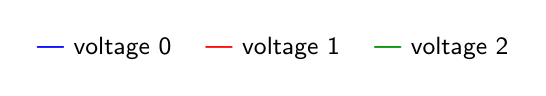
\begin{tikzpicture}[baseline]
        \node[font=\sffamily\small] at (0,0)
        {\textcolor{volt0}{\textbf{---}} voltage 0 \quad
            \textcolor{volt1}{\textbf{---}} voltage 1 \quad
        \textcolor{volt2}{\textbf{---}} voltage 2};
    \end{tikzpicture}%
}
